\chapter{Results and Analysis}\label{chap:results}

%%%%%%%%%%%%%%%%%%%%%%%%%%%%%%%%%%%%%%%%%%%%%%%%%%%%%%%%%%%%%%%%%%
%%%%%%%%%%%%%%%%%%%%%%%%%%%%%%%%%%%%%%%%%%%%%%%%%%%%%%%%%%%%%%%%%%
\section{TLS connections}
%%%%%%%%%%%%%%%%%%%%%%%%%%%%%%%%%%%%%%%%%%%%%%%%%%%%%%%%%%%%%%%%%%
%%%%%%%%%%%%%%%%%%%%%%%%%%%%%%%%%%%%%%%%%%%%%%%%%%%%%%%%%%%%%%%%%%
% Begin with the benchmark done by Bastien on the raw number of verif/s with openssl.

If the ten clients could connect instantaneously to the server every second, the maximum number of connections would be 600 per minute.
However, a certain connection time has to be taken into account.
Those are summarized in table~\ref{tab:openvpn-con-time}.

\begin{table}[ht]
\center
\small
\begin{tabular}{ll|l|} \cline{3-3}
 & & Connection time [s] \\ \hline
\multicolumn{1}{|l|}{\multirow{2}{*}{RSA-1024}} & soft & 0.041921 \\ \cline{2-3}
\multicolumn{1}{|l|}{} & BA411E & 0.020312 \\ \hline
\multicolumn{1}{|l|}{\multirow{2}{*}{RSA-2048}} & soft & 0.202945 \\ \cline{2-3}
\multicolumn{1}{|l|}{} & BA411E & 0.039965 \\ \hline
\multicolumn{1}{|l|}{\multirow{2}{*}{RSA-4096}} & soft & 1.436743 \\ \cline{2-3}
\multicolumn{1}{|l|}{} & BA411E & 0.183533 \\ \hline
\end{tabular}
\caption{OpenVPN connection time}{time necessary to establish an aes-256-cbc connection with DHE.}
\label{tab:openvpn-con-time}
\end{table}

It already shows that the connection latency is divided by 2 for low security RSA, and up to by 7.8 for higher security parameters.
The figure~\ref{fig:openvpn-tls-bench} shows the number of TLS connections per minute for three RSA exponent sizes: 1024-, 2048- and 4096-bit.
The higher the exponent size, the higher the performance boost.


\begin{table}[ht]
\center
\small
\begin{tabular}{l|c|c|c|c|c|c|c|c|c|} \cline{2-10}
 & \multicolumn{3}{c|}{RSA-1024} & \multicolumn{3}{c|}{RSA-2048} & \multicolumn{3}{c|}{RSA-4096} \\ \cline{2-10}
 & \multicolumn{2}{c|}{Con.} & CPU & \multicolumn{2}{c|}{Con.} & CPU & \multicolumn{2}{|c|}{Con.} & CPU \\ \hline
\multicolumn{1}{|c|}{Soft} & 445.4 & \multirow{2}{*}{x1.14} & 40.32 & 155.6& \multirow{2}{*}{x2.70}  & 92.14 & 19.6& \multirow{2}{*}{x5.89}  & 81.97 \\ \cline{1-2}\cline{4-5}\cline{7-8}\cline{10-10}
\multicolumn{1}{|c|}{BA414E} & 509.3 & & 13.29 & 420.9 & & 4.82 & 115.5 & & 4.34 \\ \hline
\end{tabular}
\caption{TLS connections per minute}{measures obtained with ten clients concurently connecting to an OpenVPN server.}
\label{tab:tls-con}
\end{table}

\begin{figure}[ht]
\center
\begin{tikzpicture}

%%%%%%%%%%%%%%%%%%%%%%%%
% CPU in the background
%%%%%%%%%%%%%%%%%%%%%%%%
\begin{axis}[
        width  = 0.7*\textwidth,
        height = 8cm,
        major x tick style = transparent,
        ybar=2pt,%space between the bars
        bar width=16pt,
        enlarge x limits={abs=1},
        ylabel = {CPU\#0 usage},
        hide x axis,
        axis y line*=right,
        ymin=0, ymax=100,
        symbolic x coords={RSA-1024, RSA-2048, RSA-4096},
        xtick = data,
        scaled y ticks = false,%Disable the *10^4 exponent applied to all y axis markings.
        legend style={at={(0.5,-0.15)}, anchor=north,legend columns=2},
        enlarge x limits=0.1,
    ]

\addplot[style={black,fill=LimeGreen,postaction={pattern=north east lines},mark=none}]
    coordinates {
        (RSA-1024, 40.32)
        (RSA-2048, 92.14)
        (RSA-4096, 81.97)
    };
    \label{software}

\addplot[style={black,fill=RedOrange,postaction={pattern=north east lines},mark=none}]
    coordinates {
        (RSA-1024, 13.29)
        (RSA-2048, 4.82)
        (RSA-4096, 4.78)
    };
    \label{ba414e}
\legend{software, ba414e}
\end{axis}

%%%%%%%%%%%%%%%%%%%%%%%%
% throughput
%%%%%%%%%%%%%%%%%%%%%%%%
\begin{axis}[
        title = {TLS connections through OpenVPN},
        width  = 0.7*\textwidth,
        height = 8cm,
        major x tick style = transparent,
        ybar=10pt,
        bar width=8pt,
        enlarge x limits={abs=1},
        ymajorgrids = true,
        ylabel = {Connections per minute},
        xlabel = {},
        ymin=0,
        symbolic x coords={RSA-1024, RSA-2048, RSA-4096},
        xtick = data,
        scaled y ticks = false,%Disable the *10^4 exponent applied to all y axis markings.
        legend style={at={(0.5,-0.25)}, anchor=north,legend columns=2},
        enlarge x limits=0.1,
    ]

\addplot[style={black,fill=ForestGreen,mark=none}]
    coordinates {
        (RSA-1024, 445.4)
        (RSA-2048, 155.6)
        (RSA-4096, 19.6)
    };
    \label{soft-tp}

\addplot[style={black,fill=BrickRed,mark=none}]
    coordinates {
        (RSA-1024, 509.3)
        (RSA-2048, 420.9)
        (RSA-4096, 115.5)
    };
    \label{ba411e-tp}
\legend{}
\end{axis}

\end{tikzpicture}


\caption{TLS connections per minute}{The background stripped bars are the CPU usage. Raw data in table~\ref{tab:tls-con}.}
\label{fig:openvpn-tls-bench}
\end{figure}


\noindent For RSA-1024, the results are mitigated: a poor performance increase, but already less than half the CPU usage.
It should be noted that at this point, the number of clients is probably too low to push the configuration to its limits.
It is however an interesting comparison case with the next level of security: RSA-2048.

\noindent RSA-2048 is a much more common configuration, espacially since the NIST deprecated RSA-1024 in 2013.
The full software implementation is visibly affected by the increase of the exponent size: the CPU usage doubles and the server processes three time less connections.
At the same time, the hardware loses less than 20\% connections for a third of the CPU usage.
%TODO check if it is hardware limited or limited by the performances of the VM. It is not to be forgotten that it has to keep up with the server, even when the latter is helped by the high-performance hardware. My guess is that the VM is capping the perf, hence the exact same CPU usage for RSA-2048 and RSA-4096.

\noindent The results obtained for RSA-4096 can be interpreted similarly to those of RSA-2048, except that the CPU usage is exactly the same for th hardware configuration.
One way too look at those results is to directly compare the raw performance, and the hardware can then process almost six times more connections per minute than the software.
However, this is only half of it, since it leaves the CPU usage drop aside.
If we look at the efficiency, the software can process 0.24 connection per percentage of CPU usage, whilst the hardware can process 24 of them.
The efficiency is thus multipled by a factor 1000.

Such interesting results, particularly regarding the CPU usage, are possible because at least 87\% of the operations are RSA and Diffie-Hellman operations, which are entirely offloaded in hardware.
Nevertheless, OpenVPN still needs to proceed to some extra computations (such as SHA-1 integrity), and the hardware operations are not instantaneous, so the performance gain can only be that high.












%%%%%%%%%%%%%%%%%%%%%%%%%%%%%%%%%%%%%%%%%%%%%%%%%%%%%%%%%%%%%%%%%%
%%%%%%%%%%%%%%%%%%%%%%%%%%%%%%%%%%%%%%%%%%%%%%%%%%%%%%%%%%%%%%%%%%
\section{Response time -- latency}
%%%%%%%%%%%%%%%%%%%%%%%%%%%%%%%%%%%%%%%%%%%%%%%%%%%%%%%%%%%%%%%%%%
%%%%%%%%%%%%%%%%%%%%%%%%%%%%%%%%%%%%%%%%%%%%%%%%%%%%%%%%%%%%%%%%%%
The following tests are conducted after the connection has been established, so as the clients do not need to undergo any new key negociation.

\subsection{OpenVPN}
The figure~\ref{fig:ping-benchmark-openvpn} shows the results for different payload sizes.

\noindent Firstly, is the impact of OpenVPN's operation on the delay: when no encryption nor authentication is used, the exchange is 33\% to 53\% longer. This is simply because the packet has to go through a virtual interface, hence even without the security time overhead, the latency is much longer.

When combining encryption and authentication, the software and hardware implementation are neck and neck.
Eventhough the MAC is not offload, the hardware implementation could have performed better.
The reason is not only all the packets have to go through a virtual interface in the kernel, the payload also has to be sent to the hardware through the kernel.
In the end, a packet will undergo two full round trips between the user and the kernel space, that is one more than a regular software implementation, plus a final transfer to the physical interface.

\noindent All those transfer make the offload useless in such a case in term of raw performance.
The CPU usage is not even worth mentioning as the operation is only a few milliseconds long.


\begin{figure}[ht]
%%%%%%%%%%%%%%%%%%%%%%%%%%%%%%%%%%%%%%%%%%%%%%%%%%%%%%%%%%
% Ping GCM
%%%%%%%%%%%%%%%%%%%%%%%%%%%%%%%%%%%%%%%%%%%%%%%%%%%%%%%%%%
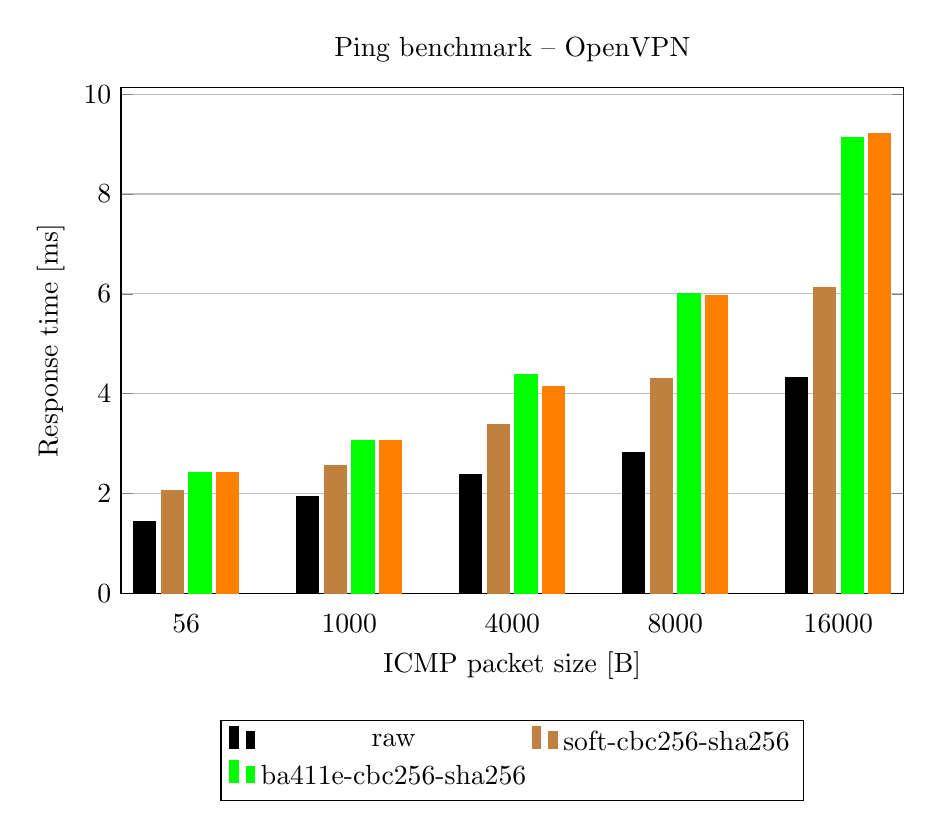
\begin{tikzpicture}
\begin{axis}[
        title = {Ping benchmark -- OpenVPN},
        width  = 0.95*\textwidth,
        height = 8cm,
        major x tick style = transparent,
        ybar,
        bar width=8pt,
        ymajorgrids = true,
        ylabel = {Response time [ms]},
        xlabel = {ICMP packet size [B]},
        ymin=0,
        symbolic x coords={56, 1000, 4000, 8000, 16000},
        xtick = data,
        scaled y ticks = false,%Disable the *10^4 exponent applied to all y axis markings.
        legend style={at={(0.5,-0.25)}, anchor=north,legend columns=2},
        enlarge x limits=0.1,
    ]
% I would have prefered to have "\addplot[marks only]", but they overlap if they have the same x coordinate,
% not like bars that automatically shift.
\addplot[style={black, fill=black}]
    coordinates {
        (56, 1.444)
        (1000, 1.929)
        (4000, 2.376)
        (8000, 2.811)
        (16000, 4.322)
    };
    \label{raw}

\addplot[style={brown, fill=brown}]
    coordinates {
        (56, 2.066)
        (1000, 2.561)
        (4000, 3.373)
        (8000, 4.293)
        (16000, 6.117)
    };
    \label{none-none}

\addplot[style={green, fill=green}]
    coordinates {
        (56, 2.415)
        (1000, 3.061)
        (4000, 4.376)
        (8000, 5.997)
        (16000, 9.135)
    };
    \label{soft-cbc256-sha256}

\addplot[style={orange, fill=orange}]
    coordinates {
        (56, 2.416)
        (1000, 3.052)
        (4000, 4.140)
        (8000, 5.963)
        (16000, 9.207)
    };
    \label{ba411e-cbc256-sha256}

\legend{raw, soft-cbc256-sha256, ba411e-cbc256-sha256}
\end{axis}
\end{tikzpicture}
% Here, I could show the gcm128, which show better performances with the BA411e, but I would be weird to compare it with aes256cbc.
% I need another graph with a CPu usage comparison to show that even if the perf are the same for soft/hard with aes256gcm, the hard loads less the CPU (I hope so, at least).
\caption{OpenVN: ping average response time}{OpenVPN adds up to 53\% extra delay and offloading the encryption does not improve the latency.}
\label{fig:ping-benchmark-openvpn}
\end{figure}

\subsection{IPsec}
The figure~\ref{fig:ping-benchmark-ipsec} studies the same payload size as OpenVPN, but with an extra experimental hardware implementation of AES mode GCM.

\noindent In this case, the time overhead imposed by IPsec is not larger than 9\%, corroborating the results of~\citet{Xenakis20063225}.

When combining encryption and authentication, the hardware implementation steadily takes the advantage over the software with the encrease of the payload length.
If they both have the same latency at default payload size, the hardware is up to 13\% faster for 16000 bytes payloads.

As for the GCM mode, the support in the BA411E driver is highly experimental and takes more of a proof of concept than a real use case.
The current implementation could not support payload sizes larger than 1000 bytes, and at this size it is 5\% faster than the software.
It is not much, but when compared to the 3\% improvement the BA411E offers at the same size for AES-256-CBC, we can expect an accelaration exceeding the 20\% for larger payload sizes. %TODO Instead of comparing with sha256, compare with none, no software holding back;
Aside from the fact that the driver is not fully working yet, it could still be extensively improved.
As an example, it still relies on the \texttt{seqiv} kernel module, as the software implementation does.
Managing the generation of the IV directly in the driver would cut it loose from yet another software boulder.

\begin{figure}[ht]
%%%%%%%%%%%%%%%%%%%%%%%%%%%%%%%%%%%%%%%%%%%%%%%%%%%%%%%%%%
% Ping GCM
%%%%%%%%%%%%%%%%%%%%%%%%%%%%%%%%%%%%%%%%%%%%%%%%%%%%%%%%%%
\begin{tikzpicture}
\begin{axis}[
        title = {Ping benchmark -- IPsec},
        width  = \textwidth,
        height = 8cm,
        major x tick style = transparent,
        ybar,
        bar width=8pt,
        ymajorgrids = true,
        ylabel = {Response time [ms]},
        xlabel = {ICMP packet size [B]},
        ymin=0, ymax=10,
        symbolic x coords={56, 1000, 8000, 16000},
        xtick = data,
        scaled y ticks = false,%Disable the *10^4 exponent applied to all y axis markings.
        legend style={at={(0.5,-0.25)}, anchor=north,legend columns=3},
        enlarge x limits=0.15,
    ]
% I would have prefered to have "\addplot[marks only]", but they overlap if they have the same x coordinate,
% not like bars that automatically shift.
\addplot[style={black, fill=black}]
    coordinates {
        (56, 1.444)
        (1000, 1.929)
        (8000, 2.811)
        (16000, 4.322)
    };
    \label{raw}

\addplot[style={NavyBlue, fill=NavyBlue}]
    coordinates {
        (56, 1.545)
        (1000, 2.045)
        (8000, 2.997)
        (16000, 4.703)
    };
    \label{none-none}

\addplot[style={OliveGreen, fill=OliveGreen},postaction={pattern=north east lines}]
    coordinates {
        (56, 1.581)
        (1000, 2.134)
        (8000, 3.910)
        (16000, 6.426)

    };
    \label{soft-cbc256-none}

\addplot[style={BrickRed, fill=BrickRed},postaction={pattern=north east lines}]
    coordinates {
        (56, 1.639)
        (1000, 2.080)
        (8000, 3.445)
        (16000, 5.345)
    };
    \label{ba411e-cbc256-none}

\addplot[style={OliveGreen, fill=OliveGreen}]
    coordinates {
        (56, 1.645)
        (1000, 2.322)
        (8000, 4.762)
        (16000, 7.975)

    };
    \label{soft-cbc256-sha256}

\addplot[style={BrickRed, fill=BrickRed}]
    coordinates {
        (56, 1.635)
        (1000, 2.246)
        (8000, 4.170)
        (16000, 6.929)
    };
    \label{ba411e-cbc256-sha256}

\addplot[style={OliveGreen, fill=OliveGreen},postaction={pattern=north west lines}]
    coordinates {
        (56, 1.651)
        (1000, 2.388)
        (8000, 5.383)
        (16000, 9.241)
    };
    \label{soft-gcm256}

\addplot[style={BrickRed, fill=BrickRed},postaction={pattern=north west lines}]
    coordinates {
        (56, 1.764)
        (1000, 2.286)
        (8000, 0)
        (16000, 0)
    };
    \label{ba411e-gcm256}

\legend{raw, none-none, soft-cbc256-none, ba411e-cbc256-none, soft-cbc256-sha256, ba411e-cbc256-sha256, soft-gcm256, ba411e-gcm256}
\end{axis}
\end{tikzpicture}
% Here, I could show the gcm256, which show better performances with the BA411e, but I would be weird to compare it with aes256cbc.
% I need another graph with a CPu usage comparison to show that even if the perf are the same for soft/hard with aes256gcm, the hard loads less the CPU (I hope so, at least).
\caption{IPsec: ping average response time}{for different packet sizes using IPsec. For each packet size, 1000 requests were flooded to the board, that is \textit{"outputs packets as fast as they come back or one hundred times per second, whichever is more"}, according to the \texttt{ping} command manual.} %TODO move the end of the caption to the "test protocol" chapter.
\label{fig:ping-benchmark-ipsec}
\end{figure}



\subsection{Comparison}
The figure~\ref{fig:ping-benchmark-comparison} summarizes the results for OpenVPN and IPsec for the most realistic use case: the combination of encryption and authentication.

\noindent The first main difference is the overhead imposed by each method: 53\% for OpenVPN and only 9\% for IPsec.
Even if those configurations are not realistic, it puts forward the advantage of directly working in the kernel as does IPsec.

As for the combination of encryption and authentication, IPsec is between 13\% and 32\% faster than OpenVPN.
IPsec loses its advantage with the increase of the payload size, the time lost when moving around the data between the user and the kernel space being less important compared to the securoty operations.

\noindent In hardware, as OpenVPN could not take advantage of the accelaration of the encryption, IPsec is even faster, ranging from 25\% to 33\% faster than OpenVPN.


\begin{figure}[ht]

\begin{tikzpicture}
\begin{axis}[
        title = {Ping benchmark},
        width  = \textwidth,
        height = 8cm,
        major x tick style = transparent,
        ybar,
        bar width=8pt,
        ymajorgrids = true,
        ylabel = {Response time [ms]},
        xlabel = {ICMP packet size [B]},
        ymin=0,
        symbolic x coords={56, 1000, 4000, 8000, 16000},
        xtick = data,
        scaled y ticks = false,%Disable the *10^4 exponent applied to all y axis markings.
        legend style={at={(0.5,-0.25)}, anchor=north,legend columns=2},
        % enlarge x limits=0.1,
    ]

\addplot[style={brown, fill=brown, postaction={pattern=north east lines}}]
    coordinates {
        (56, 1.545)
        (1000, 2.045)
        (4000, 2.521)
        (8000, 2.997)
        (16000, 4.703)
    };
    \label{ipsec-none-none}

\addplot[style={brown, fill=brown, postaction={pattern=north west lines}}]
    coordinates {
        (56, 2.066)
        (1000, 2.561)
        (4000, 3.373)
        (8000, 4.293)
        (16000, 6.117)
    };
    \label{openvpn-none-none}

\addplot[style={green, fill=green, postaction={pattern=north east lines}}]
    coordinates {
        (56, 1.645)
        (1000, 2.322)
        (4000, 3.420)
        (8000, 4.762)
        (16000, 7.975)

    };
    \label{ipsec-soft-cbc256-sha256}

\addplot[style={green, fill=green, postaction={pattern=north west lines}}]
    coordinates {
        (56, 2.415)
        (1000, 3.061)
        (4000, 4.376)
        (8000, 5.997)
        (16000, 9.135)
    };
    \label{openvpn-soft-cbc256-sha256}

\addplot[style={orange, fill=orange, postaction={pattern=north east lines}}]
    coordinates {
        (56, 1.635)
        (1000, 2.246)
        (4000, 3.172)
        (8000, 4.170)
        (16000, 6.929)
    };
    \label{ipsec-ba411e-cbc256-sha256}

\addplot[style={orange, fill=orange, postaction={pattern=north west lines}}]
    coordinates {
        (56, 2.416)
        (1000, 3.052)
        (4000, 4.140)
        (8000, 5.963)
        (16000, 9.207)
    };
    \label{openvpn-ba411e-cbc256-sha256}

\legend{ipsec-none-none, openvpn-none-none, ipsec-soft-cbc256-sha256, openvpn-soft-cbc256-sha256, ipsec-ba411e-cbc256-sha256, openvpn-ba411e-cbc256-sha256}
\end{axis}
\end{tikzpicture}
% Here, I could show the gcm256, which show better performances with the BA411e, but I would be weird to compare it with aes256cbc.
% I need another graph with a CPu usage comparison to show that even if the perf are the same for soft/hard with aes256gcm, the hard loads less the CPU (I hope so, at least).
\caption{Ping average comparison}{All values are for AES-256-CBC with SHA-256. Globally, IPsec yields better results and propose the most significant hardware offload. Quick reading: the stripped bars are the IPsec results.}
\label{fig:ping-benchmark-comparison}
\end{figure}














%%%%%%%%%%%%%%%%%%%%%%%%%%%%%%%%%%%%%%%%%%%%%%%%%%%%%%%%%%%%%%%%%%
%%%%%%%%%%%%%%%%%%%%%%%%%%%%%%%%%%%%%%%%%%%%%%%%%%%%%%%%%%%%%%%%%%
\section{File transfer}
%%%%%%%%%%%%%%%%%%%%%%%%%%%%%%%%%%%%%%%%%%%%%%%%%%%%%%%%%%%%%%%%%%
%%%%%%%%%%%%%%%%%%%%%%%%%%%%%%%%%%%%%%%%%%%%%%%%%%%%%%%%%%%%%%%%%%
%FTP over openvpn and IPsec

%OpenSSH: 	- normal transfer: shows perf difference
%			- capped to software max: show CPU offload
This use case studies the performance of a simple file transfer over three different secure implementations: OpenSSH, OpenVPN and IPsec.
For each application, three encryption:authentication couples are considered: none:none, AES-256-CBC:none and AES-256-CBC:SHA-256. 

\subsection{openSSH}

\begin{figure}[ht]
\begin{tikzpicture}

%%%%%%%%%%%%%%%%%%%%%%%%
% CPU in the background
%%%%%%%%%%%%%%%%%%%%%%%%
\begin{axis}[
        width  = 0.95*\textwidth,
        height = 8cm,
        major x tick style = transparent,
        ybar=2pt,%space between the bars
        bar width=16pt,
        enlarge x limits={abs=1},
        ylabel = {CPU\#0 usage},
        hide x axis,
        axis y line*=right,
        ymin=0, ymax=100,
        symbolic x coords={none:none, aes256cbc:none, aes256cbc:sha256},
        xtick = data,
        scaled y ticks = false,%Disable the *10^4 exponent applied to all y axis markings.
        legend style={at={(0.5,-0.15)}, anchor=north,legend columns=4},
        enlarge x limits=0.1,
    ]

\addplot[style={black,fill=LimeGreen,postaction={pattern=north east lines},mark=none}]
    coordinates {
        (none:none, 0)
        (aes256cbc:none, 96.26)
        (aes256cbc:sha256, 89.29)
    };
    \label{software}

\addplot[style={black,fill=RedOrange,postaction={pattern=north east lines},mark=none}]
    coordinates {
        (none:none, 0)
        (aes256cbc:none, 46.01)
        (aes256cbc:sha256, 68.19)
    };
    \label{ba411e}

\addplot[style={black,fill=gray,postaction={pattern=north east lines},mark=none}]
    coordinates {
        (none:none, 7.16)
        (aes256cbc:none, 0)
        (aes256cbc:sha256, 0)
    };
    \label{out-of-tunnel}%"oot" for "out of tunnel"
\legend{software, ba411e, out-of-tunnel}
\end{axis}

%%%%%%%%%%%%%%%%%%%%%%%%
% throughput
%%%%%%%%%%%%%%%%%%%%%%%%
\begin{axis}[
        title = {File transfer over an SSH tunnel},
        width  = 0.95*\textwidth,
        height = 8cm,
        major x tick style = transparent,
        ybar=10pt,
        bar width=8pt,
        enlarge x limits={abs=1},
        ymajorgrids = true,
        ylabel = {Throughtput [MB/s]},
        xlabel = {},
        ymin=0, ymax=12,
        symbolic x coords={oot, none:none, aes256cbc:none, aes256cbc:sha256},
        xtick = data,
        scaled y ticks = false,%Disable the *10^4 exponent applied to all y axis markings.
        legend style={at={(0.5,-0.25)}, anchor=north,legend columns=2},
        enlarge x limits=0.1,
    ]

\addplot[style={black,fill=ForestGreen,mark=none}]
    coordinates {
        (none:none, 0)
        (aes256cbc:none, 10.89)
        (aes256cbc:sha256, 8.19)
    };
    \label{soft-tp}

\addplot[style={black,fill=BrickRed,mark=none}]
    coordinates {
        (none:none, 0)
        (aes256cbc:none, 10.67)
        (aes256cbc:sha256, 10.39)
    };
    \label{ba411e-tp}

\addplot[style={black,fill=black,mark=none}]
    coordinates {
        (none:none, 11.39)
        (aes256cbc:none, 0)
        (aes256cbc:sha256, 0)
    };
    \label{oot-tp}%"tp" for "throughput"
\legend{}
\end{axis}

\end{tikzpicture}
\caption{file transfer over an SSH tunnel. The background stripped bars are the CPU usage.}{}
\label{fig:openssh-bench}
\end{figure}

\subsection{OpenVPN}

\begin{figure}[ht]
\begin{tikzpicture}

%%%%%%%%%%%%%%%%%%%%%%%%
% CPU in the background
%%%%%%%%%%%%%%%%%%%%%%%%
\begin{axis}[
        width  = 0.95*\textwidth,
        height = 8cm,
        major x tick style = transparent,
        ybar=2pt,%space between the bars
        bar width=16pt,
        enlarge x limits={abs=1},
        ylabel = {CPU\#0 usage},
        hide x axis,
        axis y line*=right,
        ymin=0, ymax=100,
        symbolic x coords={none:none, aes256cbc:none, aes256cbc:sha256},
        xtick = data,
        scaled y ticks = false,%Disable the *10^4 exponent applied to all y axis markings.
        legend style={at={(0.5,-0.15)}, anchor=north,legend columns=4},
        enlarge x limits=0.1,
    ]

\addplot[style={black,fill=LimeGreen,postaction={pattern=north east lines},mark=none}]
    coordinates {
        (none:none, 0)
        (aes256cbc:none, 76.60)
        (aes256cbc:sha256, 76.03)
    };
    \label{software}

\addplot[style={black,fill=RedOrange,postaction={pattern=north east lines},mark=none}]
    coordinates {
        (none:none, 0)
        (aes256cbc:none, 83.74)
        (aes256cbc:sha256, 80.89)
    };
    \label{ba411e}

\addplot[style={black,fill=gray,postaction={pattern=north east lines},mark=none}]
    coordinates {
        (none:none, 7.16)
        (aes256cbc:none, 0)
        (aes256cbc:sha256, 0)
    };
    \label{out-of-tunnel}%"oot" for "out of tunnel"

\addplot[style={black,fill=brown,postaction={pattern=north east lines},mark=none}]
    coordinates {
        (none:none, 42.60)
        (aes256cbc:none, 0)
        (aes256cbc:sha256, 0)
    };
    \label{inside tunnel}%"it" for "in tunnel"
\legend{software, ba411e, out-of-tunnel, inside tunnel}
\end{axis}

%%%%%%%%%%%%%%%%%%%%%%%%
% throughput
%%%%%%%%%%%%%%%%%%%%%%%%
\begin{axis}[
        title = {FTP transfer inside OpenVPN tunnel},
        width  = 0.95*\textwidth,
        height = 8cm,
        major x tick style = transparent,
        ybar=10pt,
        bar width=8pt,
        enlarge x limits={abs=1},
        ymajorgrids = true,
        ylabel = {Throughtput [MB/s]},
        xlabel = {},
        ymin=0, ymax=12,
        symbolic x coords={oot, none:none, aes256cbc:none, aes256cbc:sha256},
        xtick = data,
        scaled y ticks = false,%Disable the *10^4 exponent applied to all y axis markings.
        legend style={at={(0.5,-0.25)}, anchor=north,legend columns=2},
        enlarge x limits=0.1,
    ]

\addplot[style={black,fill=ForestGreen,mark=none}]
    coordinates {
        (none:none, 0)
        (aes256cbc:none, 4.78)
        (aes256cbc:sha256, 3.87)
    };
    \label{soft-tp}

\addplot[style={black,fill=BrickRed,mark=none}]
    coordinates {
        (none:none, 0)
        (aes256cbc:none, 3.35)
        (aes256cbc:sha256, 2.84)
    };
    \label{ba411e-tp}

\addplot[style={black,fill=black,mark=none}]
    coordinates {
        (none:none, 11.39)
        (aes256cbc:none, 0)
        (aes256cbc:sha256, 0)
    };
    \label{oot-tp}%"tp" for "throughput"

\addplot[style={black,fill=RawSienna,mark=none}]
    coordinates {
        (none:none, 5.18)
        (aes256cbc:none, 0)
        (aes256cbc:sha256, 0)
    };
    \label{it-tp}
\legend{}
\end{axis}

\end{tikzpicture}
\caption{FTP file transfer over an OpenVPN tunnel. The background stripped bars are the CPU usage.}{}
\label{fig:openvpn-ftp-bench}
\end{figure}

We can see that adding a MAC computation aside the encryption merely lowers the performance when using the hardware.
Even though OpenSSL uses here an hihgly ARM-optimzed assembly implementation of SHA-256, it shows that the bottleneck is on the hardware side.

Indeed, 

\subsection{IPsec}

\begin{figure}[ht]
\begin{tikzpicture}

%%%%%%%%%%%%%%%%%%%%%%%%
% CPU in the background
%%%%%%%%%%%%%%%%%%%%%%%%
\begin{axis}[
        width  = 0.95*\textwidth,
        height = 8cm,
        major x tick style = transparent,
        ybar=2pt,%space between the bars
        bar width=16pt,
        enlarge x limits={abs=1},
        ylabel = {CPU\#0 usage},
        hide x axis,
        axis y line*=right,
        ymin=0, ymax=100,
        symbolic x coords={none:none, aes256cbc:none, aes256cbc:sha256, aes256gcm},
        xtick = data,
        scaled y ticks = false,%Disable the *10^4 exponent applied to all y axis markings.
        legend style={at={(0.5,-0.15)}, anchor=north,legend columns=4},
        enlarge x limits=0.1,
    ]

\addplot[style={black,fill=LimeGreen,postaction={pattern=north east lines},mark=none}]
    coordinates {
        (none:none, 0)
        (aes256cbc:none, 63.74)
        (aes256cbc:sha256, 74.64)
        (aes256gcm, 89.66)
    };
    \label{software}

\addplot[style={black,fill=RedOrange,postaction={pattern=north east lines},mark=none}]
    coordinates {
        (none:none, 0)
        (aes256cbc:none, 14.87)
        (aes256cbc:sha256, 17.25)
        (aes256gcm, 0)
    };
    \label{ba411e}

\addplot[style={black,fill=gray,postaction={pattern=north east lines},mark=none}]
    coordinates {
        (none:none, 7.16)
        (aes256cbc:none, 0)
        (aes256cbc:sha256, 0)
        (aes256gcm, 0)
    };
    \label{out-of-tunnel}%"oot" for "out of tunnel"

\addplot[style={black,fill=NavyBlue,postaction={pattern=north east lines},mark=none}]
    coordinates {
        (none:none, 14.68)
        (aes256cbc:none, 0)
        (aes256cbc:sha256, 0)
        (aes256gcm, 0)
    };
    \label{inside tunnel}%"it" for "in tunnel"
\legend{software, ba411e, out-of-tunnel, inside tunnel}
\end{axis}

%%%%%%%%%%%%%%%%%%%%%%%%
% throughput
%%%%%%%%%%%%%%%%%%%%%%%%
\begin{axis}[
        title = {FTP transfer insed IPSec tunnel},
        width  = 0.95*\textwidth,
        height = 8cm,
        major x tick style = transparent,
        ybar=10pt,
        bar width=8pt,
        enlarge x limits={abs=1},
        ymajorgrids = true,
        ylabel = {Throughtput [MB/s]},
        xlabel = {},
        ymin=0, ymax=12,
        symbolic x coords={oot, none:none, aes256cbc:none, aes256cbc:sha256, aes256gcm},
        xtick = data,
        scaled y ticks = false,%Disable the *10^4 exponent applied to all y axis markings.
        legend style={at={(0.5,-0.25)}, anchor=north,legend columns=2},
        enlarge x limits=0.1,
    ]

\addplot[style={black,fill=ForestGreen,mark=none}]
    coordinates {
        (none:none, 0)
        (aes256cbc:none, 8.83)
        (aes256cbc:sha256, 6.47)
        (aes256gcm, 5.09)
    };
    \label{soft-tp}

\addplot[style={black,fill=BrickRed,mark=none}]
    coordinates {
        (none:none, 0)
        (aes256cbc:none, 8.52)
        (aes256cbc:sha256, 5.80)
        (aes256gcm, 0)
    };
    \label{ba411e-tp}

\addplot[style={black,fill=black,mark=none}]
    coordinates {
        (none:none, 11.39)
        (aes256cbc:none, 0)
        (aes256cbc:sha256, 0)
        (aes256gcm, 0)
    };
    \label{oot-tp}%"tp" for "throughput"

\addplot[style={black,fill=MidnightBlue,mark=none}]
    coordinates {
        (none:none, 10.21)
        (aes256cbc:none, 0)
        (aes256cbc:sha256, 0)
        (aes256gcm, 0)
    };
    \label{it-tp}
\legend{}
\end{axis}

\end{tikzpicture}
\caption{FTP file transfer over an IPsec tunnel. The background stripped bars are the CPU usage.}{}
\label{fig:ipsec-ftp-bench}
\end{figure}

Some results have to be put into perspective with the fact that the implementation of SHA-256 is entirely C-based.
A more recent one using assembly instructions optimized for the NEON SIMD instruction set of the ARMv7 core could be used and would most probably yield better results.
The CPU usage of the software implementation would drop -- even if not significantly -- as for the hardware, it would be less limited by the software MAC counter part, and if the CPU usage could stay at the same level, we could expect a better throughput.

The GCM performance presented clearly shows a drop of throughput and an increase of CPU usage, illustrating the fact that those operations are hard on the software.
With an hardware offload, we could expect not only a drastic drop of the CPU usage, but an increase of throughput as well, since it's CPU-limited in those results.
Note that they are achieved usinf a C-based implementation of galois-field multiplications.
As we saw in chapter~\ref{chap:theory}, modern processor designers tend to add specialized instruction set aimed at AES-GCM enhancement.
Should further tests be conducted concerning IPsec paired with GCM, it would be wise to compare with an assembly implementation exploiting ARM NEON instruction set.
Some are being developed~\cite{Conrado2013,Danilo2013}, but none have been committed to the Linux kernel repository yet.

\subsection{Comparison}

\begin{figure}[ht]
\begin{tikzpicture}

%%%%%%%%%%%%%%%%%%%%%%%%
% CPU in the background
%%%%%%%%%%%%%%%%%%%%%%%%
\begin{axis}[
        width  = 0.95*\textwidth,
        height = 8cm,
        major x tick style = transparent,
        ybar=2pt,%space between the bars
        bar width=16pt,
        enlarge x limits={abs=1},
        ylabel = {CPU\#0 usage},
        hide x axis,
        axis y line*=right,
        ymin=0, ymax=100,
        symbolic x coords={Out-of-tunnel, openSSH, OpenVPN, IPSec},
        xtick = data,
        scaled y ticks = false,%Disable the *10^4 exponent applied to all y axis markings.
        legend style={at={(0.5,-0.15)}, anchor=north,legend columns=4},
        enlarge x limits=0.1,
    ]

\addplot[style={black,fill=LimeGreen,postaction={pattern=north east lines},mark=none}]
    coordinates {
        (Out-of-tunnel, 0)
        (openSSH, 89.29)
        (OpenVPN, 76.03)
        (IPSec, 74.64)
    };
    \label{software-cpu}

\addplot[style={black,fill=RedOrange,postaction={pattern=north east lines},mark=none}]
    coordinates {
        (Out-of-tunnel, 0)
        (openSSH, 68.29)
        (OpenVPN, 80.89)
        (IPSec, 17.25)
    };
    \label{ba411e-cpu}

\addplot[style={black,fill=gray,postaction={pattern=north east lines},mark=none}]
    coordinates {
        (Out-of-tunnel, 7.16)
        (openSSH, 0)
        (OpenVPN, 0)
        (IPSec, 0)
    };
    \label{out-of-tunnel-cpu}%"oot" for "out of tunnel"
\end{axis}

%%%%%%%%%%%%%%%%%%%%%%%%
% throughput
%%%%%%%%%%%%%%%%%%%%%%%%
\begin{axis}[
        title = {Comparison over file transfer methods},
        width  = 0.95*\textwidth,
        height = 8cm,
        major x tick style = transparent,
        ybar=10pt,
        bar width=8pt,
        enlarge x limits={abs=1},
        ymajorgrids = true,
        ylabel = {Throughput [MB/s]},
        xlabel = {},
        ymin=0, ymax=12,
        symbolic x coords={Out-of-tunnel, openSSH, OpenVPN, IPSec},
        xtick = data,
        scaled y ticks = false,%Disable the *10^4 exponent applied to all y axis markings.
        legend style={at={(0.5,-0.15)}, anchor=north,legend columns=4},
        enlarge x limits=0.1,
    ]

\addplot[style={black,fill=ForestGreen,mark=none}]
    coordinates {
        (Out-of-tunnel, 0)
        (openSSH, 8.19)
        (OpenVPN, 3.87)
        (IPSec, 6.47)
    };
    \label{software}

\addplot[style={black,fill=BrickRed,mark=none}]
    coordinates {
        (Out-of-tunnel, 0)
        (openSSH, 10.39)
        (OpenVPN, 2.84)
        (IPSec, 5.80)
    };
    \label{ba411e}

\addplot[style={black,fill=black,mark=none}]
    coordinates {
        (Out-of-tunnel, 11.39)
        (openSSH, 0)
        (OpenVPN, 0)
        (IPSec, 0)
    };
    \label{out-of-tunnel}%"tp" for "throughput"
\legend{software, ba411e, out-of-tunnel}
\end{axis}

\end{tikzpicture}
\caption{Comparison of file transfer methods}{The background stripped bars are the CPU usage.}
\label{fig:ftp-bench-comparison}
\end{figure}